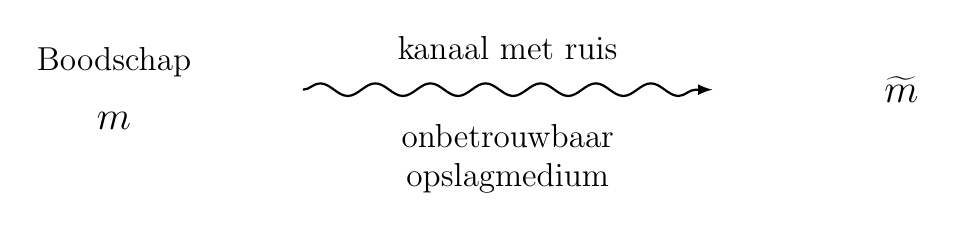
\begin{tikzpicture}[
    >=latex,
    textline/.style={
        font=\large,
        align=center
    },
    formula/.style={
        font=\Large
    },
    noisy channel/.style={
        ->,
        thick,
        decorate,
        decoration={
            snake,
            amplitude=0.8mm,
            segment length=7mm,
            post length=2mm
        }
    }
]

% Horizontal positions
\def\MessageX{0}
\def\ChannelStart{2.4}
\def\ChannelEnd{7.6}
\def\OutputX{10}

% Original message
\node[textline] at (\MessageX,0.75)
    {Boodschap};

\node[formula] at (\MessageX,0)
    {$m$};

% Noisy channel
\draw[noisy channel]
    (\ChannelStart,0.4)
    --
    node[
        above=7pt,
        textline
    ]
    {kanaal met ruis}
    node[
        below=9pt,
        textline
    ]
    {onbetrouwbaar\\opslagmedium}
    (\ChannelEnd,0.4);

% Possibly corrupted message
\node[formula] at (\OutputX,0.4)
    {$\widetilde{m}$};

\end{tikzpicture}